\subsection{RNA Synthesis}\label{sec:RNA_synthesis}
With the machinery governing the replication of the genome accounted for, we
now turn our attention to the next stage of the central dogma -- the
transcription of DNA to form RNA. We consider three major groupings
of RNA, namely the RNA associated with ribosomes (rRNA), the RNA encoding the
amino-acid sequence of proteins (mRNA), and the RNA which links codon
sequence to amino-acid identity during translation (tRNA).

rRNA serves as the catalytic and structural
framework along with myriad ribosomal proteins as part of a complete ribosomal complex.
Each ribosome contains three rRNA molecules of lengths 120, 1542,
and 2904 nucleotides (BNID: 108093), meaning each ribosome
contains $\approx$ 4500 nucleotides overall. As the \textit{E. coli} RNA polymerase
transcribes DNA to RNA at a rate of $\approx$ 40 nucleotides per second
(BNID: 101904), it takes a single RNA polymerase
$\approx$ 100 s to synthesize the RNA needed to form a single functional ribosome.
% Therefore, in a 5000 s division time, a single RNA polymerase transcribing
% rRNA at a time would result in only $\approx$ 50 functional ribosomal rRNA
% units -- far below the observed number of $\approx 10^4$ ribosomes per cell.
% Of course, there can be more than one RNA polymerase transcribing the rRNA genes
% at any given time.
Rather than rely on an estimate for the number of ribosomes needed per cell
(an estimate we consider in depth towards the end of this work), we will aim
to elucidate the \textit{maximum} number of rRNA units that can
be synthesized given the 7 copies of the rRNA genes present on the \textit{E.
coli} chromosome (BNID: 100352). To do so, we will imagine that each rRNA operon is completely
tiled with RNA polymerase. 
\textit{In vivo} measurements of the kinetics of rRNA transcription have revealed that
RNA polymerases are loaded onto the promoter of an rRNA gene at a rate of
$\approx$ 1 per second (BNID: 111997, 102362). If RNA
polymerases are constantly loaded at this rate,
then we can assume that $\approx$ 1 functional rRNA unit is
synthesized per second per rRNA operon. While \textit{E. coli} possesses 7
of these operons per chromosome (5 of which are located closely to the origin of
replication), the fact that chromosome
replication can be parallelized means that the average dosage of rRNA genes can
be in the range of 10 to 70 copies per cell at fast growth rates. At a growth
rate of $\approx$ 0.5 hr$^{-1}$, the average cell has $\approx$ 1 copy of its
chromosome and therefore approximately $\approx$ 7 copies of the rRNA operons,
therefore producing $\approx$ 7 rRNA units per second. 
At fast growth rates, this can be
further increased as multiple copies of the chromosome will be present per cell,
yielding large rRNA gene dosages between 10 and 70 copies per cell.
With a 5000 second division time, this means the cell is able to generate around 3 $\times$ 10$^4$ functional rRNA units,
comparable within an order of magnitude to the number of ribosomes per cell.


% With a 5000 second division time, this hypothesis
% leads to a maximal value of 5000 functional rRNA units, actually undershooting
% the observed number of $10^4$ ribosomes per cell.
%\textit{E. coli}, like many other bacterium, have evolved a clever mechanism to surpass this kinetic limit
%for the rate of rRNA production. Rather than having only one copy of each rRNA
%gene, \textit{E. coli} has seven copies of the operon (BIND: 100352) four of which are localized directly adjacent to the origin of
%replication \citep{birnbaum1971}. As fast growth, with
%  this also implies an increased gene
% dosage due to
%parallelized chromosomal replication, the total number of rRNA genes can be on
%the order of $\approx$ 10 -- 70 copies \citep{stevenson2004}.  Given a 5000
%second division time, we can make the lower-bound estimate that the typical cell
%will have $\approx$ 7 copies of the rRNA operon. Synthesizing one functional
%rRNA unit per second per rRNA operon, a total of $5 \times 10^4$ rRNA units can
%be synthesized, comfortably above the observed number of ribosomes per cell.

How many RNA polymerases are then needed to constantly transcribe 7 copies of
the rRNA genes? If one polymerase is loaded per second, and the transcription
rate is $\approx$ 40 nucleotides per second, then the the typical spacing
between polymerases will be $\approx$ 40 nucleotides. However, we must note that
the polymerase itself has a footprint of $\approx$ 40 nucleotides (BNID: 107873), meaning that
one could expect to find one RNA polymerase per 80 nucleotide stretch of an rRNA
gene.  With a total length of
$\approx$ 4500 nucleotides per operon and 7 operons per cell, the maximum
number of RNA polymerases that can be transcribing rRNA at any given time is then
$\approx$ 500 per cell.

The synthesis of rRNA demands the majority share of the required RNA polymerase
per cell. As outlined in \FIG{RNA_synthesis}, and discussed further the Appendix
\nameref{sec:SI_central_dogma}, synthesis of mRNA and tRNA together require on
the order of $\approx$ 400 RNAP. Thus, in total, one would expect the typical
cell to require $\approx$ 1000 RNAP to satisfy its transcriptional demands.
As is revealed in \FIG{RNA_synthesis}(B), this estimate is about an order of magnitude below the
observed number of RNA polymerase complexes per cell ($\approx$ 5000 - 7000).
The difference between the estimated number of RNA polymerase needed for
transcription and and these observations are consistent with recent literature
revealing that $\approx$ 80 \% of RNA polymerases in \textit{E. coli} are not
transcriptionally active \citep{patrick2015}. 

Our estimate neglects other mechanitic features of transcription and
transcriptional initiation more broadly. For example, we acknowledge that some
fraction of the RNAP pool is nonspecifically bound to DNA searching for a
promoter from which to begin transcription. Furthermore, we ignore 
the obstacles that RNA polymerase and DNA polymerase present for each other at
they move along the DNA \citep{finkelstein2013}. Finally, we neglect the fact
that, while they are the machinery for transcription, RNA polymerase is not
sufficient to initiate transcription. Promoter recognition and initiation of
transcription is dependent on the presence of $\sigma$-factors, proteinaceous
cofactors which bind directly to the polymerase \citep{browning2016}. In
\FIGSUPP[RNA_synthesis]{sigma_70}, we show that the predicted RNA polymerase
copy number is more comparable wit the abundance of $\sigma$-70 (RpoD), the
primary sigma factor in \textit{E. coli}. There remains more to be investigated as  to what sets the observed abundance of
RNA polymerase in these proteomic data sets.

%. However, we conclude that our
%the observed excess in abundance for RNA polymerase 
%abundances are generally in excess of what appears to be needed for growth, suggesting
%that the abundance of RNA polymerase itself is not particularly limiting.

%It is also vital to consider the role of $\sigma$-factors which
%help RNA polymerase identify and bind to transcriptional start sites
%\citep{browning2016}. Here we consider $\sigma^{70}$ (RpoD) which is the
%dominant "general-purpose" $\sigma$-factor in \textit{E. coli}. While initially
%thought of as being solely involved in transcriptional initiation, the past two
%decades of single-molecule work has revealed a more multipurpose role for
%$\sigma^{70}$ including facilitating transcriptional elongation
%\citep{kapanidis2005, goldman2015, perdue2011,mooney2003,mooney2005}.
%\FIGSUPP[RNA_synthesis]{sigma_70} is suggestive of such a role as the number of
%$\sigma^{70}$ proteins per cell is in close agreement with our estimate of the
%number of transcriptional complexes needed.

%These estimates provide insight as to the observed magnitude of both RNA
%polymerase and the $\sigma$-70 factor.
% As we have done in the previous sections,
% and described in Appendix \nameref{sec:SI_continuum_est}, we can generalize these estimates
% across a wide range of growth rates (grey line in \FIG{RNA_synthesis}(B).
% estimate appears to very adequately describe the growth rate dependence of these
% complexes. Furthermore, these findings illustrate that transcription
% cannot be the rate limiting step in bacterial division. \FIG{RNA_synthesis} (A)
% reveals that the availability of RNA polymerase is not a limiting factor for
% cell division as the cell always has an apparent $\sim$ 10-fold excess than needed.
% Furthermore, if more transcriptional activity was needed to satisfy the cellular
% requirements, more $\sigma^{70}$-factors could be expressed to utilize a larger
% fraction of the RNA polymerase pool.



\begin{figure}
    \centering{
        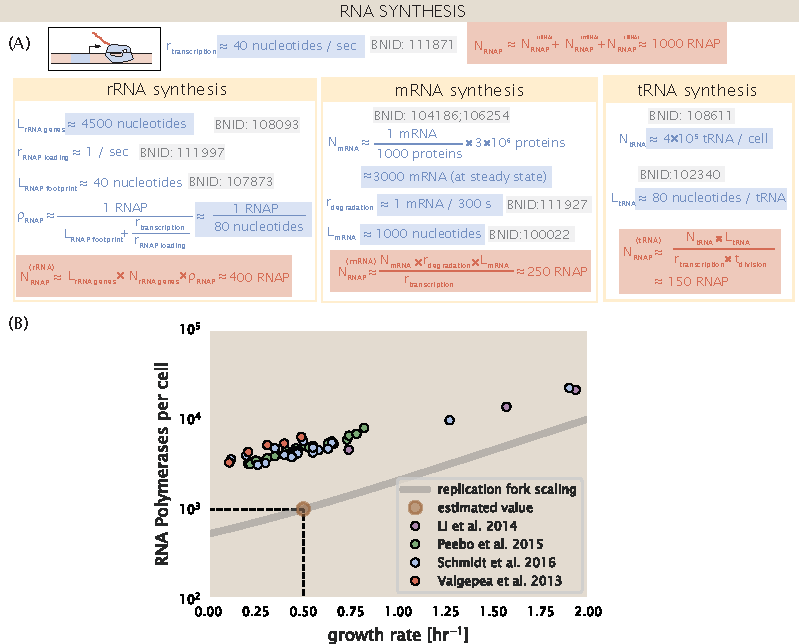
\includegraphics{main_figs/RNA_synthesis_main.pdf}
    }
        \caption{\textbf{Estimation of the RNA polymerase demand and
        comparison with experimental data.} (A) Estimations for the number of
        RNA polymerase needed to synthesize sufficient quantities of rRNA, mRNA,
        and tRNA from left to right, respectively.(B) The RNA
        polymerase core enzyme copy number as a function of growth rate. Colored
        points correspond to the average number RNA polymerase core enzymes that
        could be formed given a subunit stoichiometry of
        [RpoA]$_2$[RpoC][RpoB].} \label{fig:RNA_synthesis}

        \figsupp[Abundance and growth rate dependence of $\sigma$-70.]{The abundance of $\sigma^{70}$ as a function of growth rate.
        Estimated value for the number of RNAP is shown as a translucent brown
        point and grey line.}{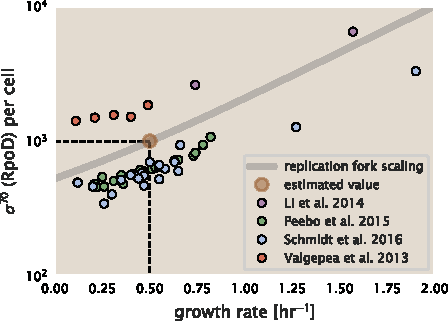
\includegraphics{main_figs/sigma_factor.pdf}}\label{figsupp:sigma_70}

\end{figure}
